\section{Data Collection}
\label{sec:data}

\begin{figure*}[h]
	\centering
	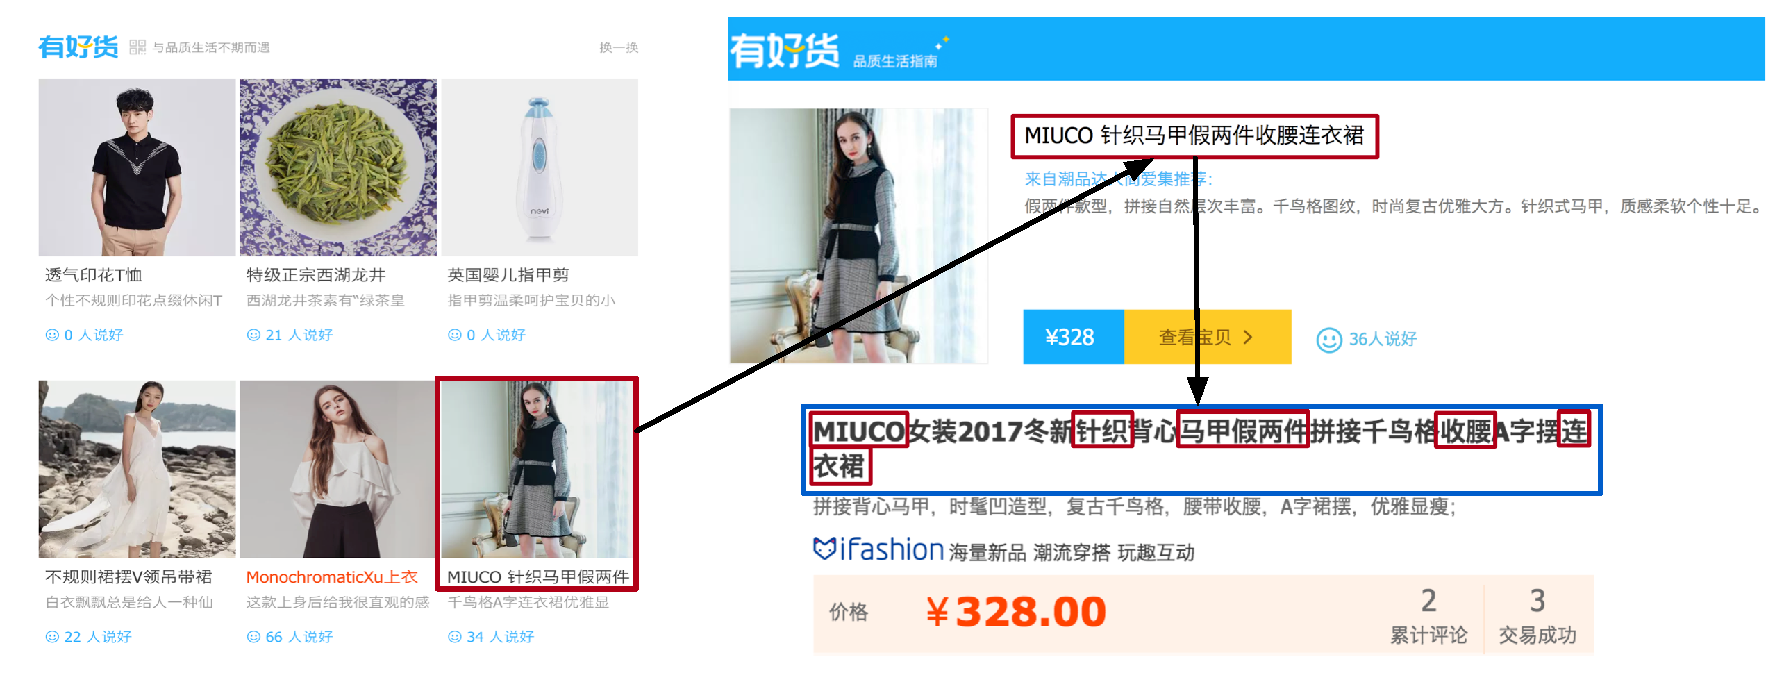
\epsfig{file=fig/youhaohuo_demo.eps, angle=0, width=2\columnwidth}
	\caption{Procedure of data collection in Youhaohuo.}
	\label{fig:youhaohuo_demo}
	\vspace{-10pt}
\end{figure*}

%Recently, deep learning methods have shown potential abilities
%to learn summarization (including extractive or abstractive methods) \cite{cheng2016neural,narayan2017neural,rush2015neural}.
%Data-driven neural summarization models require a large training corpus of
%documents (or sentences) with labels indicating which sentences (or terms) should be in the summary.
Publicly available large-scale summarization dataset is rare.
Existing document summarization datasets include
DUC2\footnote{\url{http://duc.nist.gov/data.html}}, 
TAC3\footnote{\url{http://www.nist.gov/tac/2015/KBP/}} and 
TREC4\footnote{\url{http://trec.nist.gov/}} for English,
and LCSTS\footnote{\url{http://icrc.hitsz.edu.cn/Article/show/139.html}} for
Chinese.
In this work, we create a dataset on short title extraction for 
E-commerce products. 
This dataset comes from a module in \textbf{Taobao} named ``有好货''(Youhaohuo)\footnote{\url{https://h5.m.taobao.com/lanlan/index.html}}.
{\em Youhaohuo} is a collection of high-quality 
products on Taobao.  If you click a product in Youhaohuo, you will 
be redirected to the detailed product page (including product title).
What is different from ordinary Taobao products is that online merchants are 
required to submit a short title for each Youhaohuo product.
This short title, written by humans, is readable and describes the 
key properties of the product.
Furthermore, most of these short titles are directly extracted from the 
original product titles. 
Thus, we believe Youhaohuo is a good data source of 
extractive summarization for product descriptions.

%In this work, we collect and clean the data from Youhaohuo to a publishing standard and will soon make it public.
%Each entry of this dataset contanis an manully extracted short title paired with its corresponding original long title.
%We conduct several extractive summarization experiments on this dataset, which will be introduced in the following sections.
%For the abstractive summary dataset, in which online merchants may generate new words or phrases in the short titles,
%we will collect and release it in our future work.

\figref{fig:youhaohuo_demo} shows how we collected the data.
On the left is a web page in Youhaohuo displaying several products, 
each of which contains an image and a short title below. 
When clicking on the bottom right dress, we jump to the detailed page 
on the right.  The title next to the picture in red box is the manually 
written short title, which says ``MIUCO针织马甲假两件收腰连衣裙'' (MIUCO tight dress with knit vest).
This short title is extracted from the long title below in the blue box. 
Notice that all the characters in the short tile are directly extracted from 
the long title (red boxes inside blue box). 
In addition to the characters in the short title, the long title also 
contains extra information such as ``女装2017冬新'' (woman's wear brand new
in winter 2017). In this work, we segment the original long titles and 
short titles into Chinese words by jieba~\footnote{\url{https://pypi.python/pypi/jieba/}}.

%(put in intro) The long title describe the detailed information about the product while the short title contains only most essential words for customers to grab a basic idea of the product.

The dataset consists of 6,481,623 pairs of original and short product titles, 
which is the largest short text summarization dataset to date.
We call it large extractive summary dataset for E-commerce (LESD4EC),
whose statistics is shown in \tabref{tab:data}.
We believe this dataset will contribute to the future research of
short text summarization.~\footnote{The dataset will be published after
the paper is accepted. Notice all the original data can be crawled online.}.

\begin{table}[th]
	\centering
	\scriptsize
	\caption{Statistics of LESD4EC dataset.}
	\label{tab:data}
	\begin{tabular}{l|r}
		\toprule
		%  & XXX \\ %& LCSTS  \\
		% \midrule
		No. of summaries & 6,481,623 \\%& 2,400,591  \\
		\midrule
		No. of words per text  & 12 \\ %& 60 \\
		\midrule
		No. of chars per text & 27  \\ %& 105 \\
		\midrule
		No. of words per summary & 5  \\ %& 10  \\
		\midrule
		No. of chars per summary & 11  \\ %& 19 \\
		%\midrule
		%Domain & E-commerce  \\ %& News \\
		%\midrule
		%Human annotation & 100\%\\ %& Partially \\
		\bottomrule
	\end{tabular}
	\vspace{-10pt}
\end{table}

